\documentclass[border={10pt, 10pt, 10pt, 10pt}]{standalone}

\usepackage{tikz}
\usepackage{graphicx}
\usepackage{varwidth}

\renewcommand\familydefault{\sfdefault}

\begin{document}
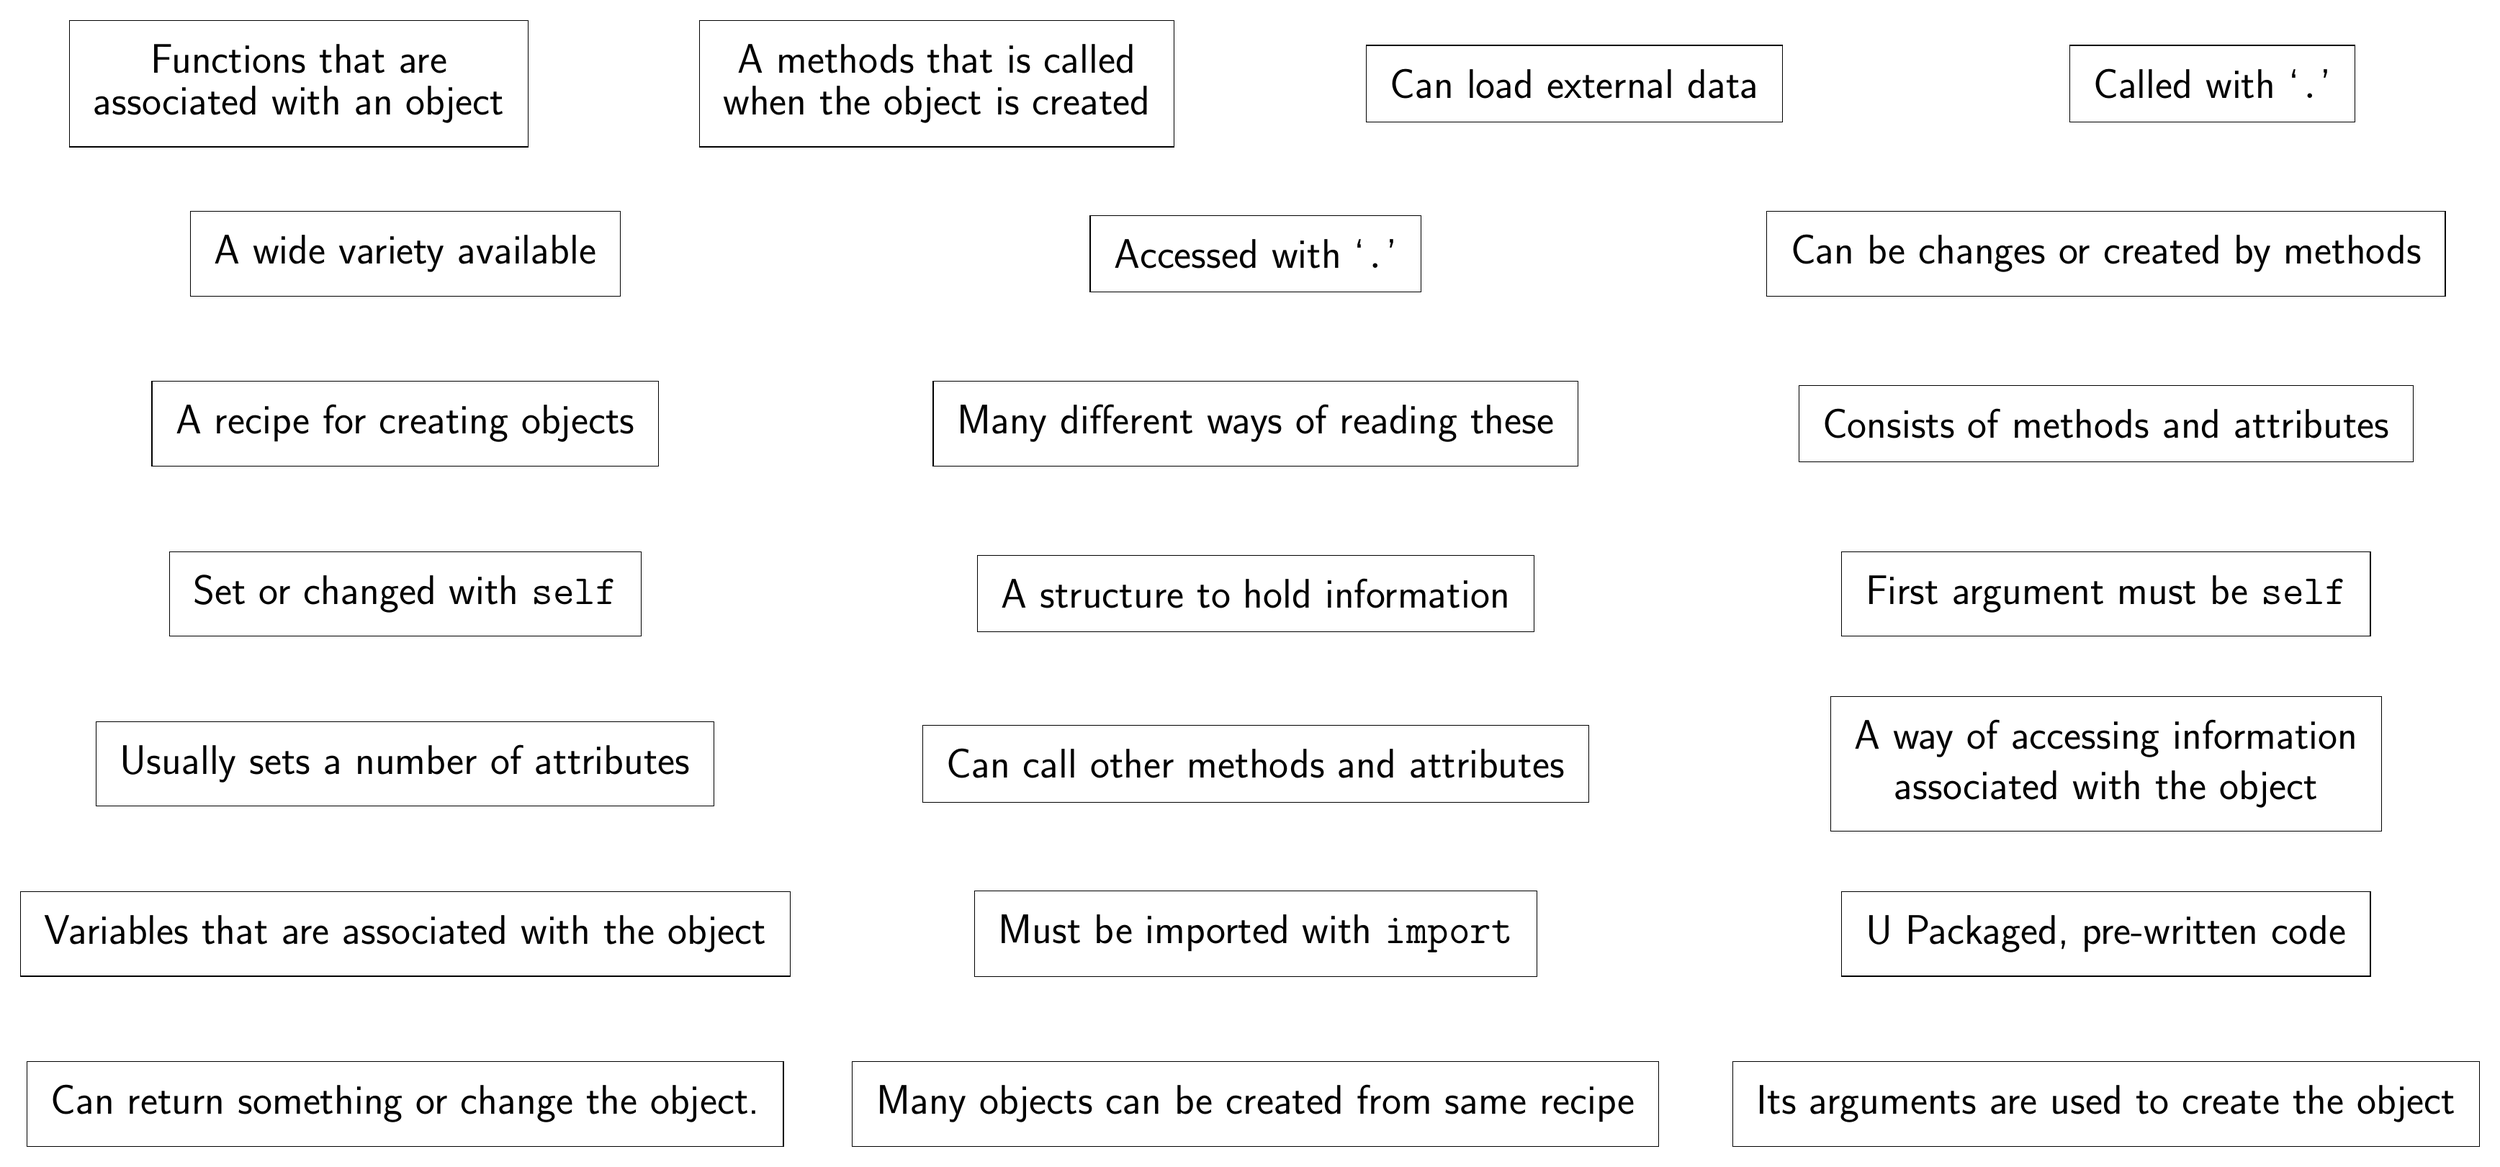
\begin{tikzpicture}
\node[align=center, draw=black, inner sep=12] at (0, 0) {\huge Can return something or change the object.};
\node[align=center, draw=black, inner sep=12] at (15, 0) {\huge Many objects can be created from same recipe};
\node[align=center, draw=black, inner sep=12] at (30, 0) {\huge Its arguments are used to create the object};
\node[align=center, draw=black, inner sep=12] at (0, 3) {\huge Variables that are associated with the object};
\node[align=center, draw=black, inner sep=12] at (15, 3) {\huge Must be imported with \texttt{import}};
\node[align=center, draw=black, inner sep=12] at (30, 3) {\huge U Packaged, pre-written code};
\node[align=center, draw=black, inner sep=12] at (0, 6) {\huge  Usually sets a number of attributes};
\node[align=center, draw=black, inner sep=12] at (15, 6) {\huge Can call other methods and attributes};
\node[align=center, draw=black, inner sep=12] at (30, 6) {\huge A way of accessing information\\[2mm]\huge associated with the object};
\node[align=center, draw=black, inner sep=12] at (0, 9) {\huge Set or changed with \texttt{self}};
\node[align=center, draw=black, inner sep=12] at (15, 9) {\huge A structure to hold information};
\node[align=center, draw=black, inner sep=12] at (30, 9) {\huge First argument must be \texttt{self}};
\node[align=center, draw=black, inner sep=12] at (0, 12) {\huge A recipe for creating objects};
\node[align=center, draw=black, inner sep=12] at (15, 12) {\huge Many different ways of reading these};
\node[align=center, draw=black, inner sep=12] at (30, 12) {\huge Consists of methods and attributes};
\node[align=center, draw=black, inner sep=12] at (0, 15) {\huge A wide variety available};
\node[align=center, draw=black, inner sep=12] at (15, 15) {\huge Accessed with `\texttt{.}'};
\node[align=center, draw=black, inner sep=12] at (30, 15) {\huge  Can be changes or created by methods};
\node[align=center, draw=black, inner sep=12] at (-1.875, 18) {\huge Functions that are\\[2mm]\huge associated with an object};
\node[align=center, draw=black, inner sep=12] at (9.375, 18) {\huge A methods that is called\\[2mm]\huge when the object is created};
\node[align=center, draw=black, inner sep=12] at (20.625, 18) {\huge Can load external data};
\node[align=center, draw=black, inner sep=12] at (31.875, 18) {\huge Called with `\texttt{.}'};

\end{tikzpicture}
\end{document}